\documentclass[11pt, a4paper]{article}

% Encoding and Language
\usepackage[utf8]{inputenc}
% \usepackage[main=english, spanish]{babel}  catalan?

% Margins
\usepackage[margin=2.5cm]{geometry}
% Line Spacing
\usepackage{setspace}

% Mathematics
\usepackage{amsmath} % Splits equations
\usepackage{amssymb} % Additional symbols
% \usepackage{cancel} % To cancel terms, if needed

% Graphics
\usepackage{graphicx} % For including images

% Tables
\usepackage{booktabs} % For better tables
\usepackage{multirow} % For multi-row cells
\usepackage{longtable} % For tables that span pages
\usepackage{float} % To prevent repositioning of tables
\restylefloat{table}
\usepackage{array} % For math mode in tables

% Units and Uncertainty
\usepackage{siunitx} % Better units and uncertainties
\sisetup{inter-unit-product = \ensuremath{{}\cdot{}}, separate-uncertainty = true}

%  Special (greek) characters
\usepackage{bookmark}

% Bibliography
\usepackage[sorting=none]{biblatex}
\usepackage{csquotes}

% Hyperlinks
% \usepackage[bookmarks,breaklinks,colorlinks=true,allcolors=blue]{hyperref}

% Custom Table Names in Spanish
% \addto\captionsspanish{
%     \def\tablename{Tabla}
%     \def\listtablename{Índice de tablas}
% }

\addbibresource{references.bib}

\begin{document}

    % \begin{titlepage}
    
    \vspace*{5mm}
    \begin{figure}[h!]
    
\includegraphics[width=6.5cm]{Images/logo.pdf}
    \end{figure}
    
    {
    \fontfamily{qhv}\selectfont
    \vspace{15mm}
    \raggedright
    \LARGE\textbf{FINAL DEGREE PROJECT}\\
    \vspace{25mm}
    
    \raggedleft
    \LARGE\textbf{EFFECT OF BACTERIAL CHEMOTAXIS ON NUTRIENT UPTAKE BY THE CHEMOATTRACTOR CELL}\\
    \vspace{30mm}
    
    \raggedright
    \LARGE\textbf{Jorge Pottiez López-Jurado}\\
    \vspace{12mm}
    \large\textbf{Degree in Physics}\\
    \vspace{7mm}
    \large\textbf{Faculty of Science}\\
    \vspace{20mm}
    \normalsize\textbf{Academic year 2024-25}\\
    }
\end{titlepage}

{
\newpage
\thispagestyle{empty}
\mbox{}
\newpage
}

\begin{titlepage}
    {
    \fontfamily{qhv}\selectfont
    \raggedright
    \vspace*{17mm}
    \hspace{1cm}\LARGE\textbf{
        EFFECT OF CHEMOTAXIS ON NUTRIENT UPTAKE \\ 
        \hspace{1cm} BY THE CHEMOATTRACTOR CELL}\\
    \vspace{29mm}

    \hspace{10mm}\LARGE\textbf{Jorge Pottiez López-Jurado}\\
    \vspace{7mm}
    \hspace{1cm}\LARGE\textbf{Final Degree Project}\\
    \vspace{7mm}
    \hspace{1cm}\Large\textbf{Faculty of Physics}\\
    \vspace{7mm}
    \hspace{1cm}\Large\textbf{University of the Balearic Islands}\\
    \vspace{7mm}
    \hspace{1cm}\normalsize\textbf{Academic Year 2024-25}\\
    \vspace{17mm}

    \hspace{1cm}\small\textbf{Keywords:}\\
    \vspace{3mm}
    \hspace{1cm}\small Biophysics, Microbiology, \\
    \hspace{1cm}\small Diffusion, Stochasticity.\\
    \vspace{25mm}

    \hspace{1cm}\large\textit{Thesis Supervisor's Name: \_\_\_\_\_\_}\\
    \vspace{1cm}
    \hspace{1cm}\large\textit{Tutor's Name (if applicable): \_\_\_\_\_\_}\\
    
    \vspace{22mm}
    \hspace{0.5cm}
    \parbox[b]{3.8in}{
        \fontfamily{qhv}\selectfont \small
        The University is hereby authorized to include this project in its institutional repository for its open consultation and online dissemination, for academic and research purposes only.
        }
    \hspace{1.9cm}
    
\includegraphics[scale=0.2]{Images/tik_cross_blank.png}
    }
\end{titlepage}

{
\newpage
\thispagestyle{empty}
\mbox{}
\newpage
}

    \hypersetup{linkcolor= black}
    \tableofcontents
    \newpage

    % Set Line Spacing to 1.5
    \onehalfspacing

    \section{Introduction}
    \subsection*{Hook}


{\color{red}
Our complex reality reveals itself as a limit for our compartmentalisation of knowledge,
that is why I believe we should increase communication between different fields of science.
Moreover, in an interdisciplinarity context, physics as a lot to offer.
This work is a personal exercise towards this philosophy. 
}
\subsection*{Research Aim}

What is the impact on the transport of nitrates to non-motile phytoplankton cells (diatoms) in
the presence of chemotactic bacteria?

\subsection*{Objectives}

\begin{itemize}
    \item Quantifying the impact of bacterial chemotaxis on the diatom's nutrient availability.
    \item Modelling the nutrient transport dynamics: Diffusion Equation with a Consumption term.
    \item Implementing a numerical solution for the model.
    \item Analytical results validating the numeric's.
    \item \color{red} Qualify which symbiotic relationship exists between bacterium and the diatom.  
\end{itemize}




\vspace{1cm}

\textit{Hook w Background}

    \newpage

    \section{Literature Review}
    \subsection{Biological Background}

\subsubsection*{Overview of Phytoplankton and Their Role in Ecosystems}

\begin{itemize}
    \item Role of phytoplankton in aquatic ecosystems (Contribution to the food chain, O2 production and CO2 absorption).
    \item Importance of Nitrate Nutrients (Phytoplankton growth and nutrient uptake mechanisms, Emergence of competition due to nutrient limitation).
\end{itemize}

\subsubsection*{Bacterium: Competitors in Nutrient Uptake}

\begin{itemize}
    \item Chemotaxis mechanisms (Foraging strategy for marine (and soil) microorganisms)
    \item Competition (Chemotactic bacteria are attracted to and consume nitrates, competing with diatoms for nutrient availability).
\end{itemize}

\subsubsection*{Interaction with Bacteria: Competition for Nitrates and Symbiosis}

\begin{itemize}
    \item Diatoms secrete chemicals that attract bacteria.
    \item \color{red} ¿Optimization of bacterial chemotaxis by diatoms?
\end{itemize}

    \section{Methodology}
    % \subsection{Theoretical Framework: A Continuum Model}
\subsection{From Discreet to Continuum}

\subsubsection*{Chemotaxis at an Individual Level}

\begin{itemize}
    \item Discreet and stochastic model.
    \item Individual trajectory, \( x_j(t) \).
\end{itemize}\subsubsection*{Chemotaxis at a Population Level}

\begin{itemize}
    \item Transition from individual to population-level, discrete to continuum approaches.
    \item Continuum and deterministic model, diffusion equation with consumption.
    \item Concentration, \( c(t) \).
\end{itemize}

\subsection{Non-Dimensionalisation}

We start from the physical equation, where we have capitalised its magnitudes:
\begin{equation}
    \frac{\partial N(\vec{R}, T)}{\partial T} =
    D \, \nabla^2_{\vec{R}} \, N(\vec{R}, T)
    - \mathrm{A} \, N(\vec{R}, T) \,C(\vec{R}, T)
\label{eq:Diff_physical}
\end{equation}

These quantities represent the real, laboratory measures:
\(\vec{R}\) is the position vector relative to the diatom,
\(T\) is time,
\(D\) is the diffusion coefficient,
\(N\) \& \(C\) are the nutrient and bacterial concentration respectively, and
\(\mathrm{A}\) is the bacterial consumption rate.
Now, we introduce the following variables changes, to obtain a dimensionless equation:

\begin{equation}
\left\{
    \vec{R} = L \, \vec{r}, \
    T = \frac{L^2}{D} \, t, \quad
    N = \frac{n}{L^3}, \quad
    C = \frac{c}{L^3}, \quad
    \mathrm{A} = DL \, \alpha
\right\}
\label{eq:change_of_vars}
\end{equation}

Where the set of lowercase variables (like \(n\) or \(\alpha\)) are the dimensionless equivalent of the capitalised variables. 
Whereas \(L\) represents the characteristic length of the system (for example, the system's or diatom's size),
\(\frac{L^2}{D}\) is the time unit of the system, meaning the time it takes for a nutrient to diffuse through \(L\). 
Replacing these (\ref{eq:change_of_vars}) into the equation (\ref{eq:Diff_physical}),
we obtain the new equation (\ref{eq:Diff_non-dim}) which is ideal for numerical simulations.

\begin{equation}
    \frac{\partial n (\vec{r}, t)}{\partial t} =
    \nabla^2_{\vec{r}} \, n (\vec{r}, t)
    - \alpha \, n(\vec{r}, t) \, c(\vec{r}, t)
\label{eq:Diff_non-dim}
\end{equation}

    \newpage
    
    \section{Results}
    \subsection{One-Dimensional Model}

\subsubsection{Diffusion With Consumption}

\textbf{Different Bacterial Concentrations}

\begin{figure}[H]
    \centering
    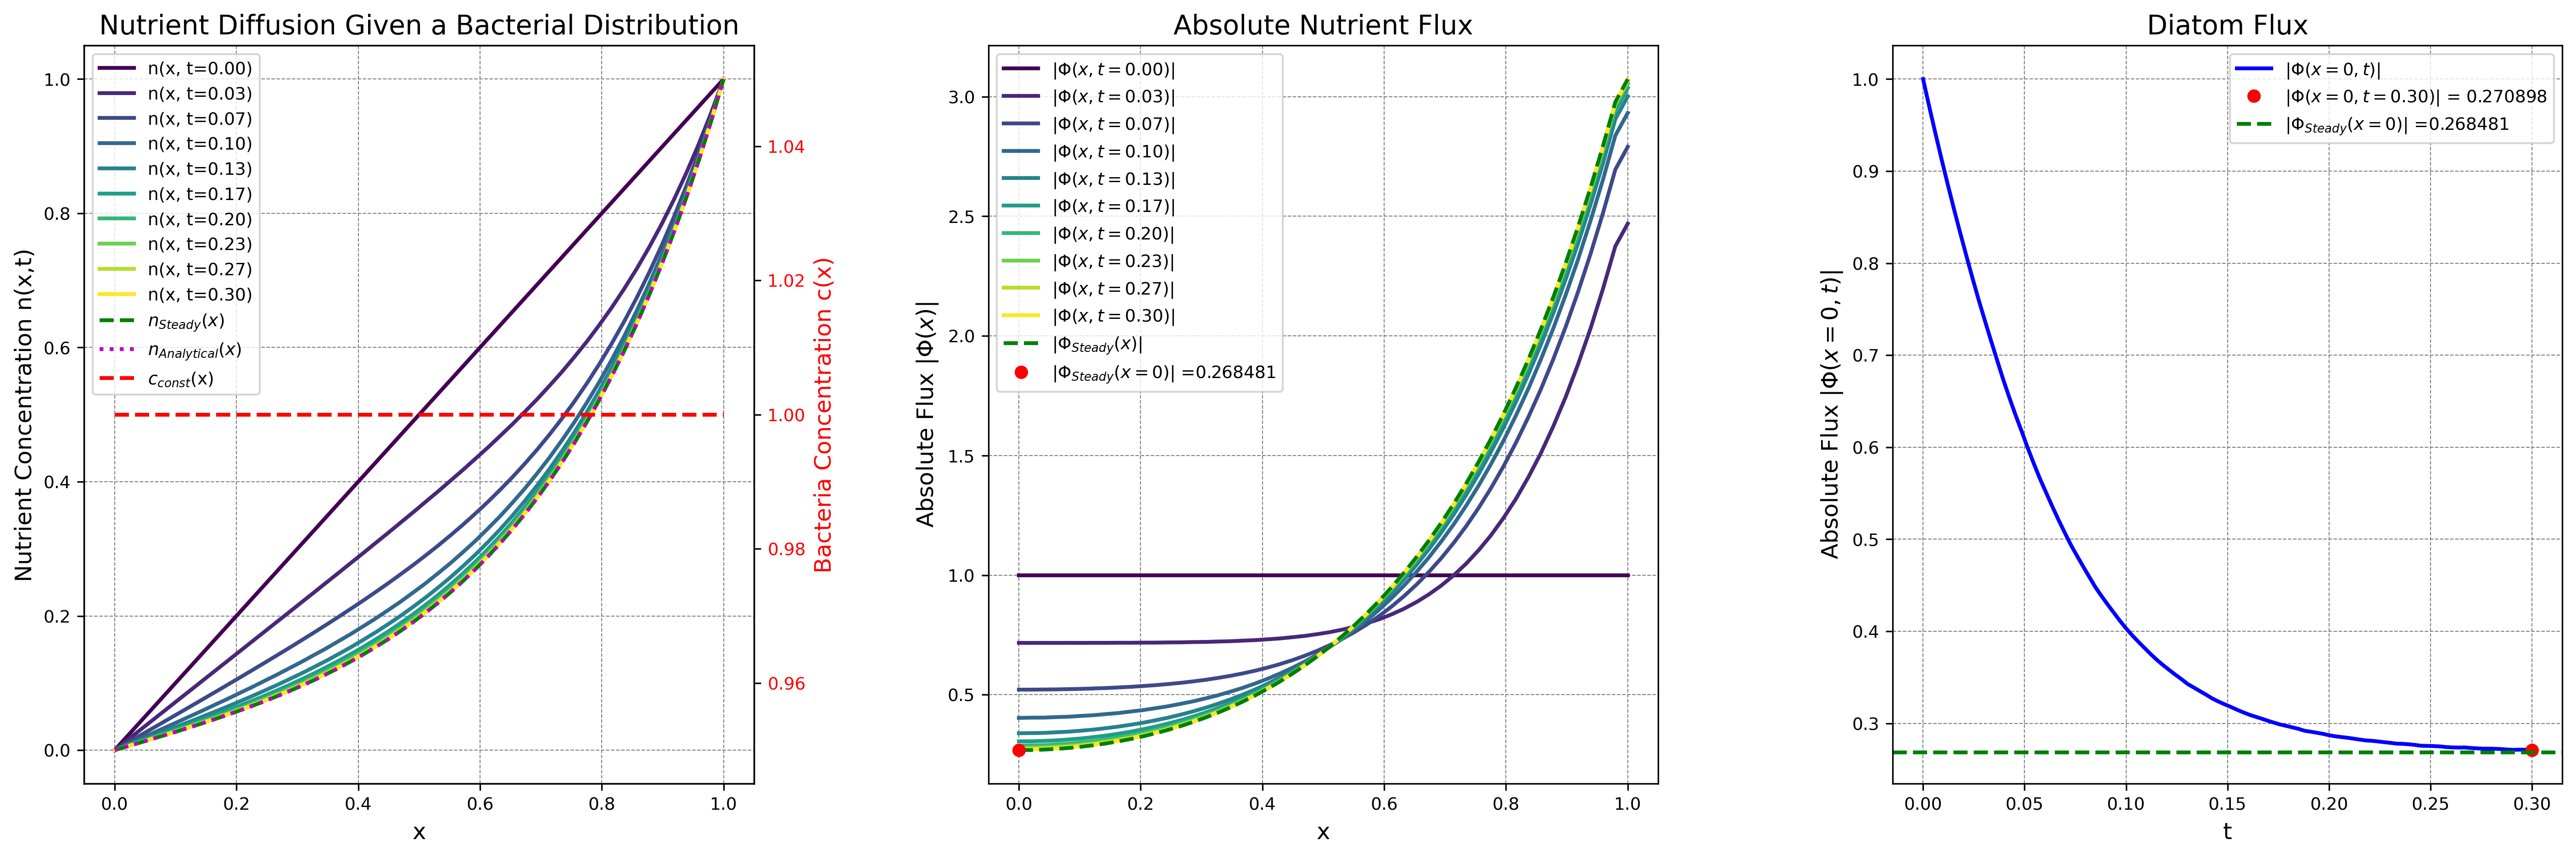
\includegraphics[width=0.8\textwidth]{Figures/c_const(x)_Analyt.png}
    \caption{Constant Bacterial Concentration Profile, with Analytical Solution.}
    \label{fig:c_const}
\end{figure}

\begin{figure}[H]
    \centering
    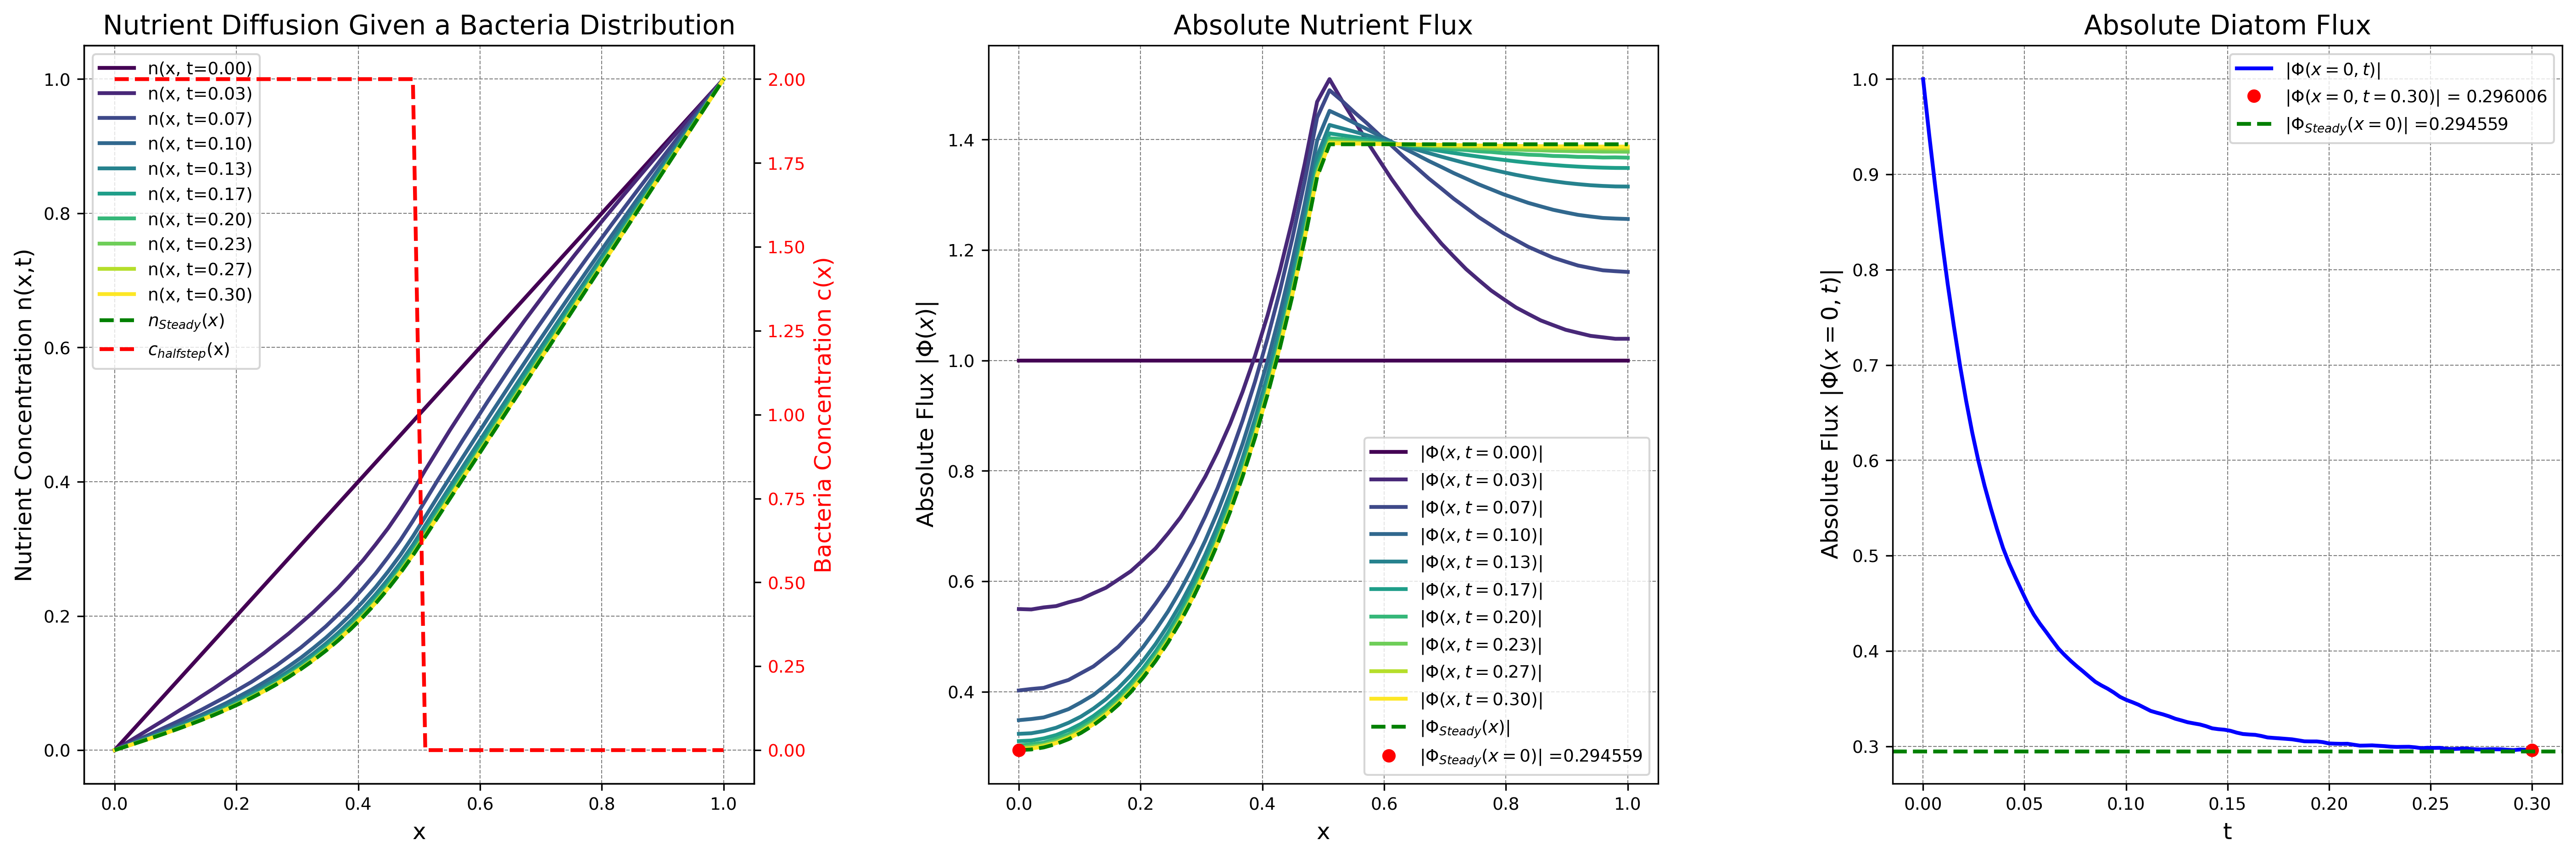
\includegraphics[width=0.8\textwidth]{Figures/c_halfstep(x).png}
    \caption{Half-Step Bacterial Concentration Profile.}
    \label{fig:c_halfstep}
\end{figure}

\begin{figure}[H]
    \centering
    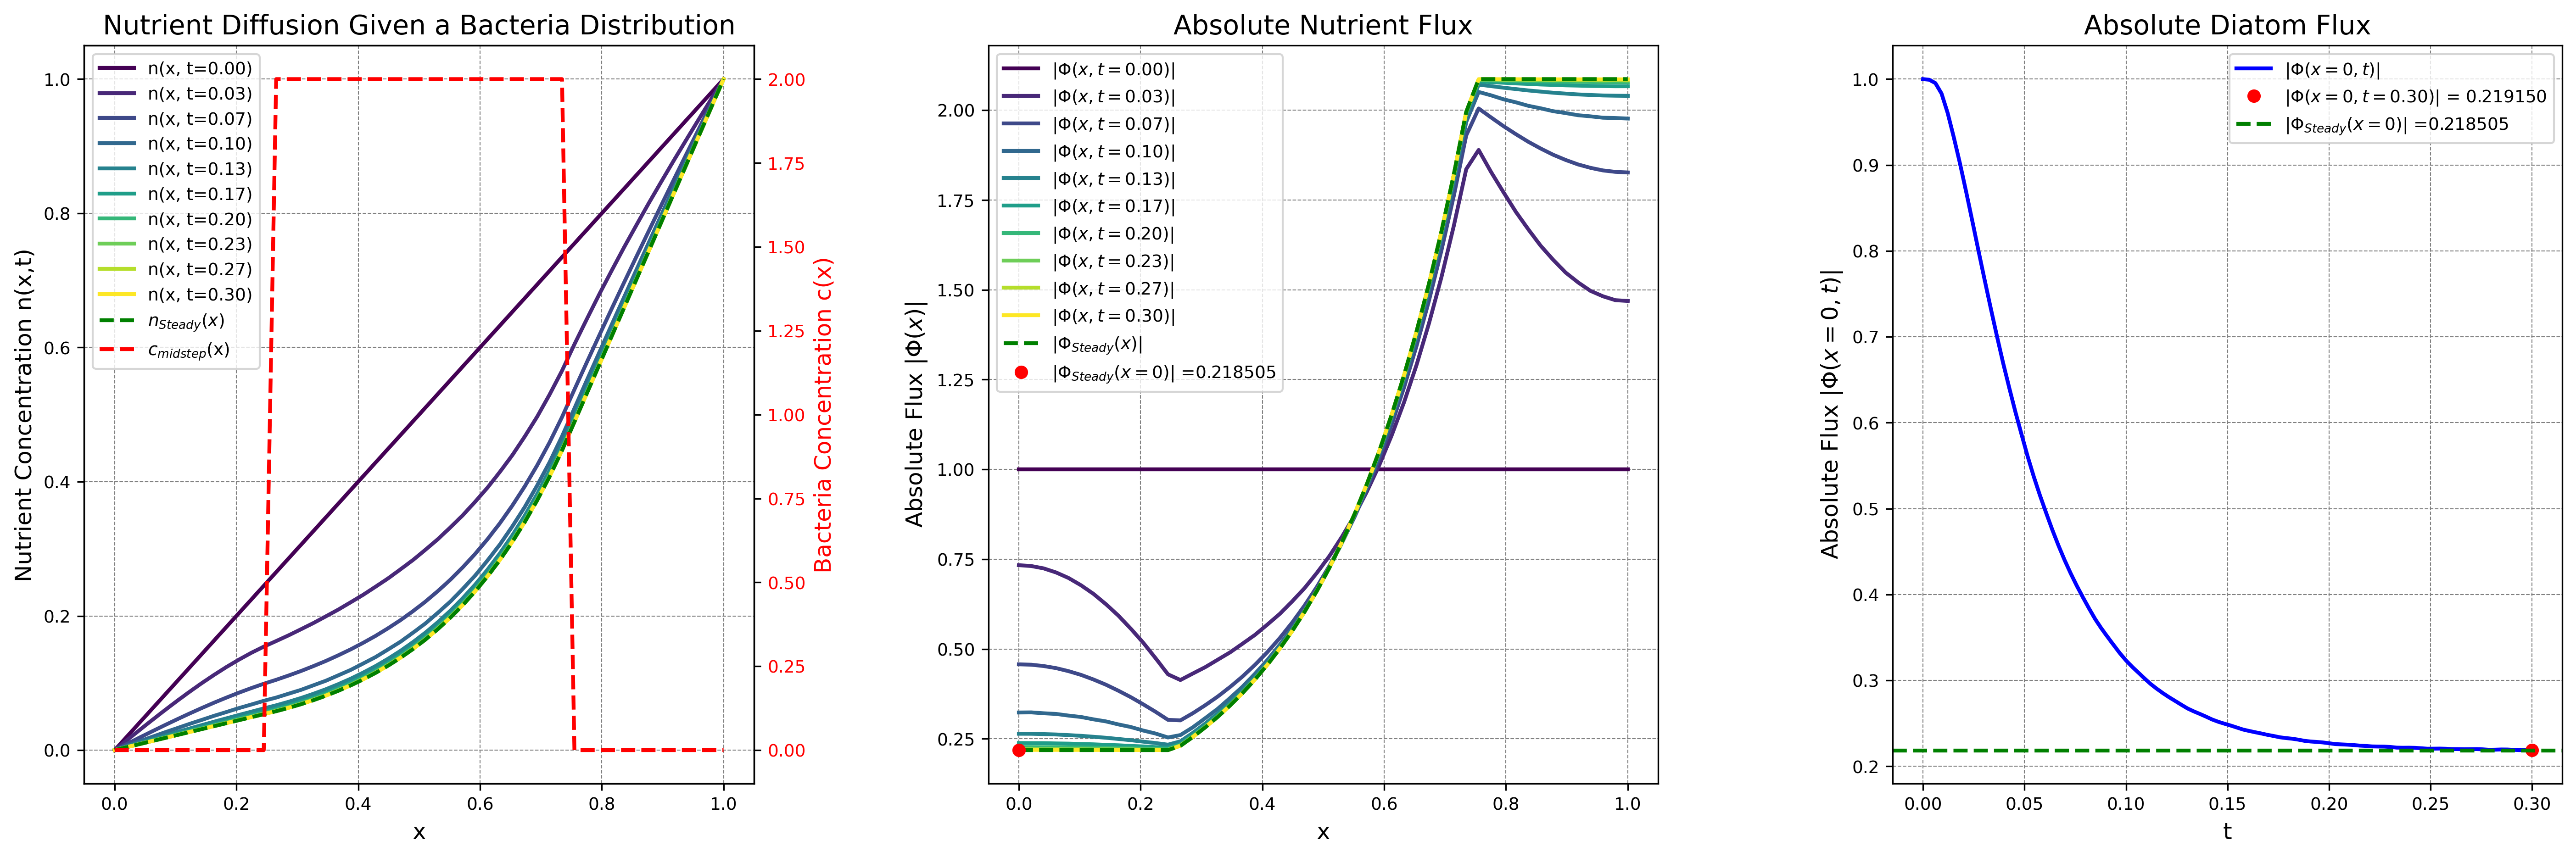
\includegraphics[width=0.8\textwidth]{Figures/c_midstep(x).png}
    \caption{Mid-Step Bacterial Concentration Profile.}
    \label{fig:c_midstep}
\end{figure}

\textbf{ \color{red} ¿Different Diffusion Coefficients?}

\begin{figure}[H]
    \centering
    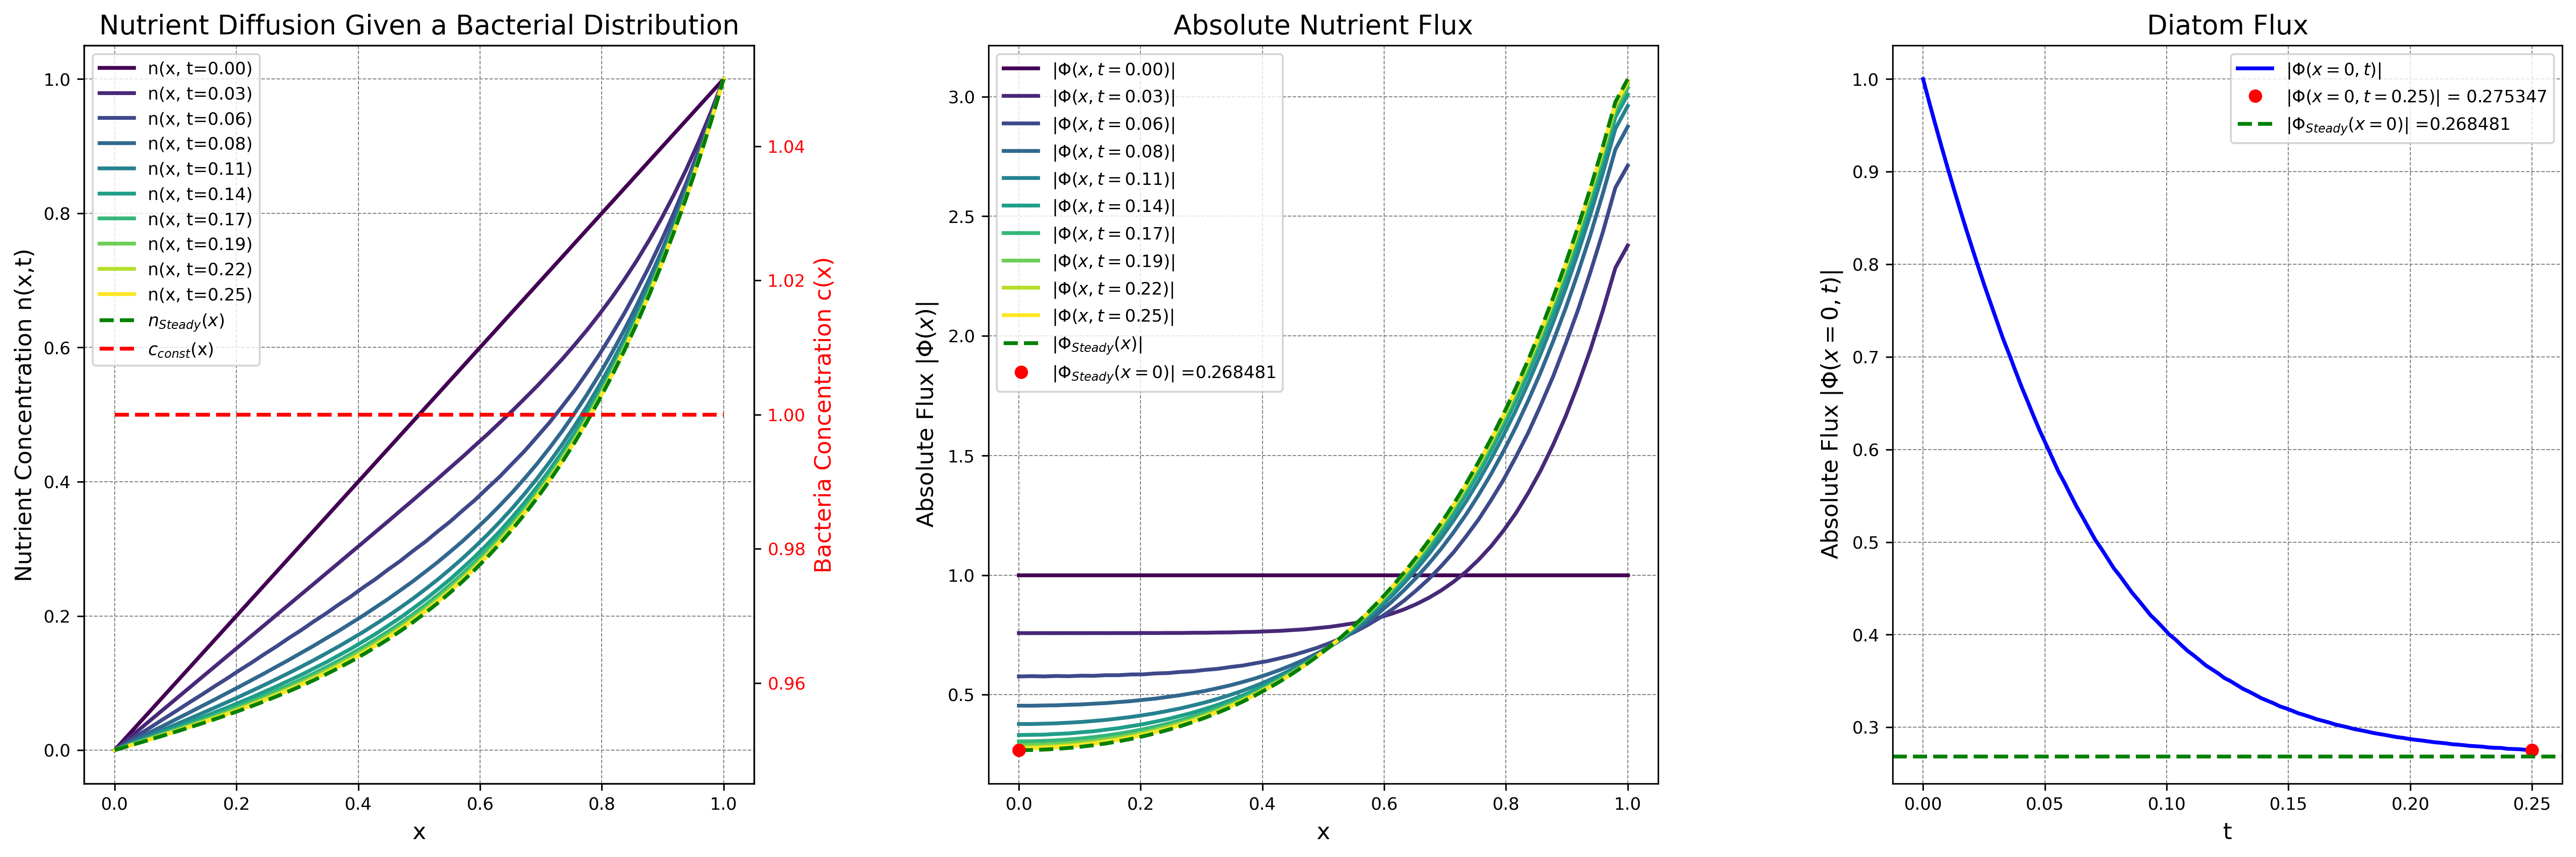
\includegraphics[width=0.8\textwidth]{Figures/Diff_Dom.png}
    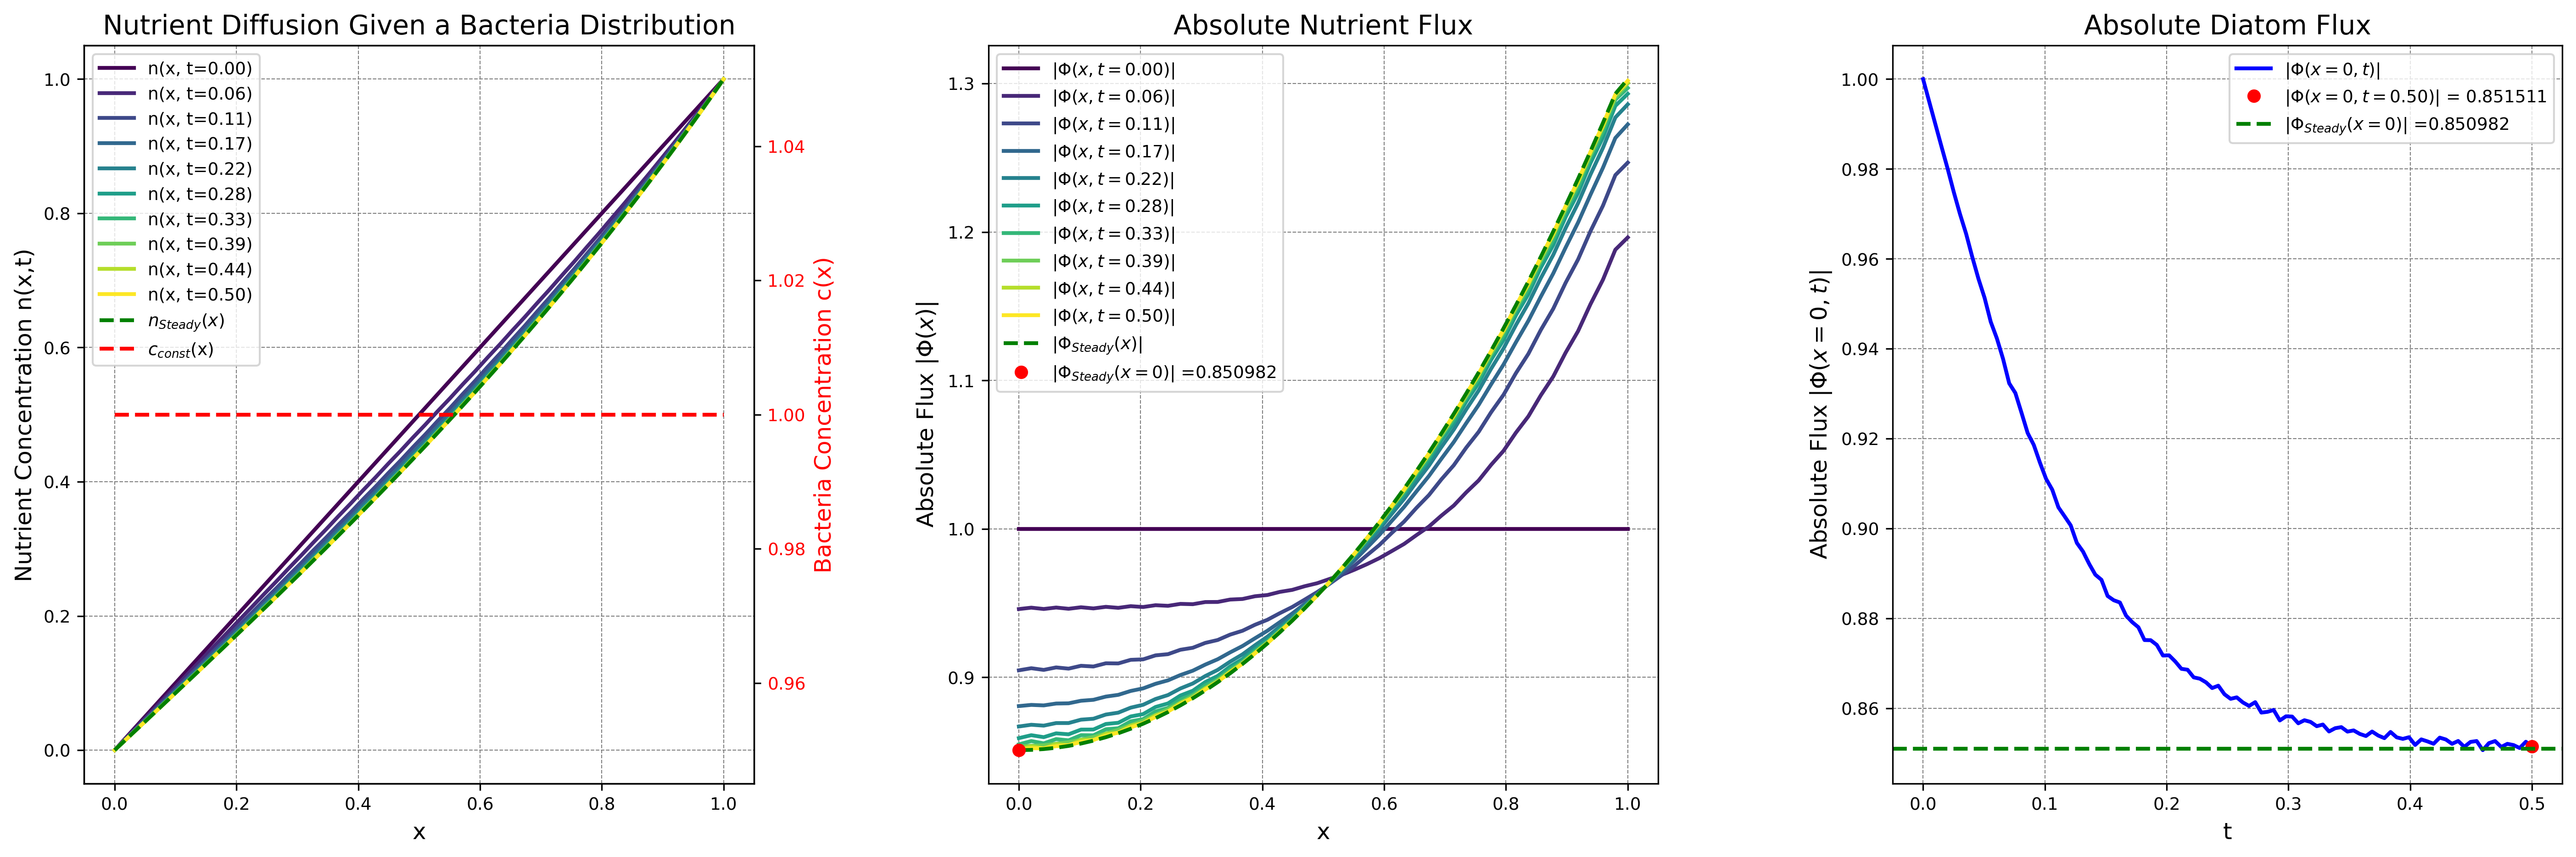
\includegraphics[width=0.8\textwidth]{Figures/Diff~Consump.png}
    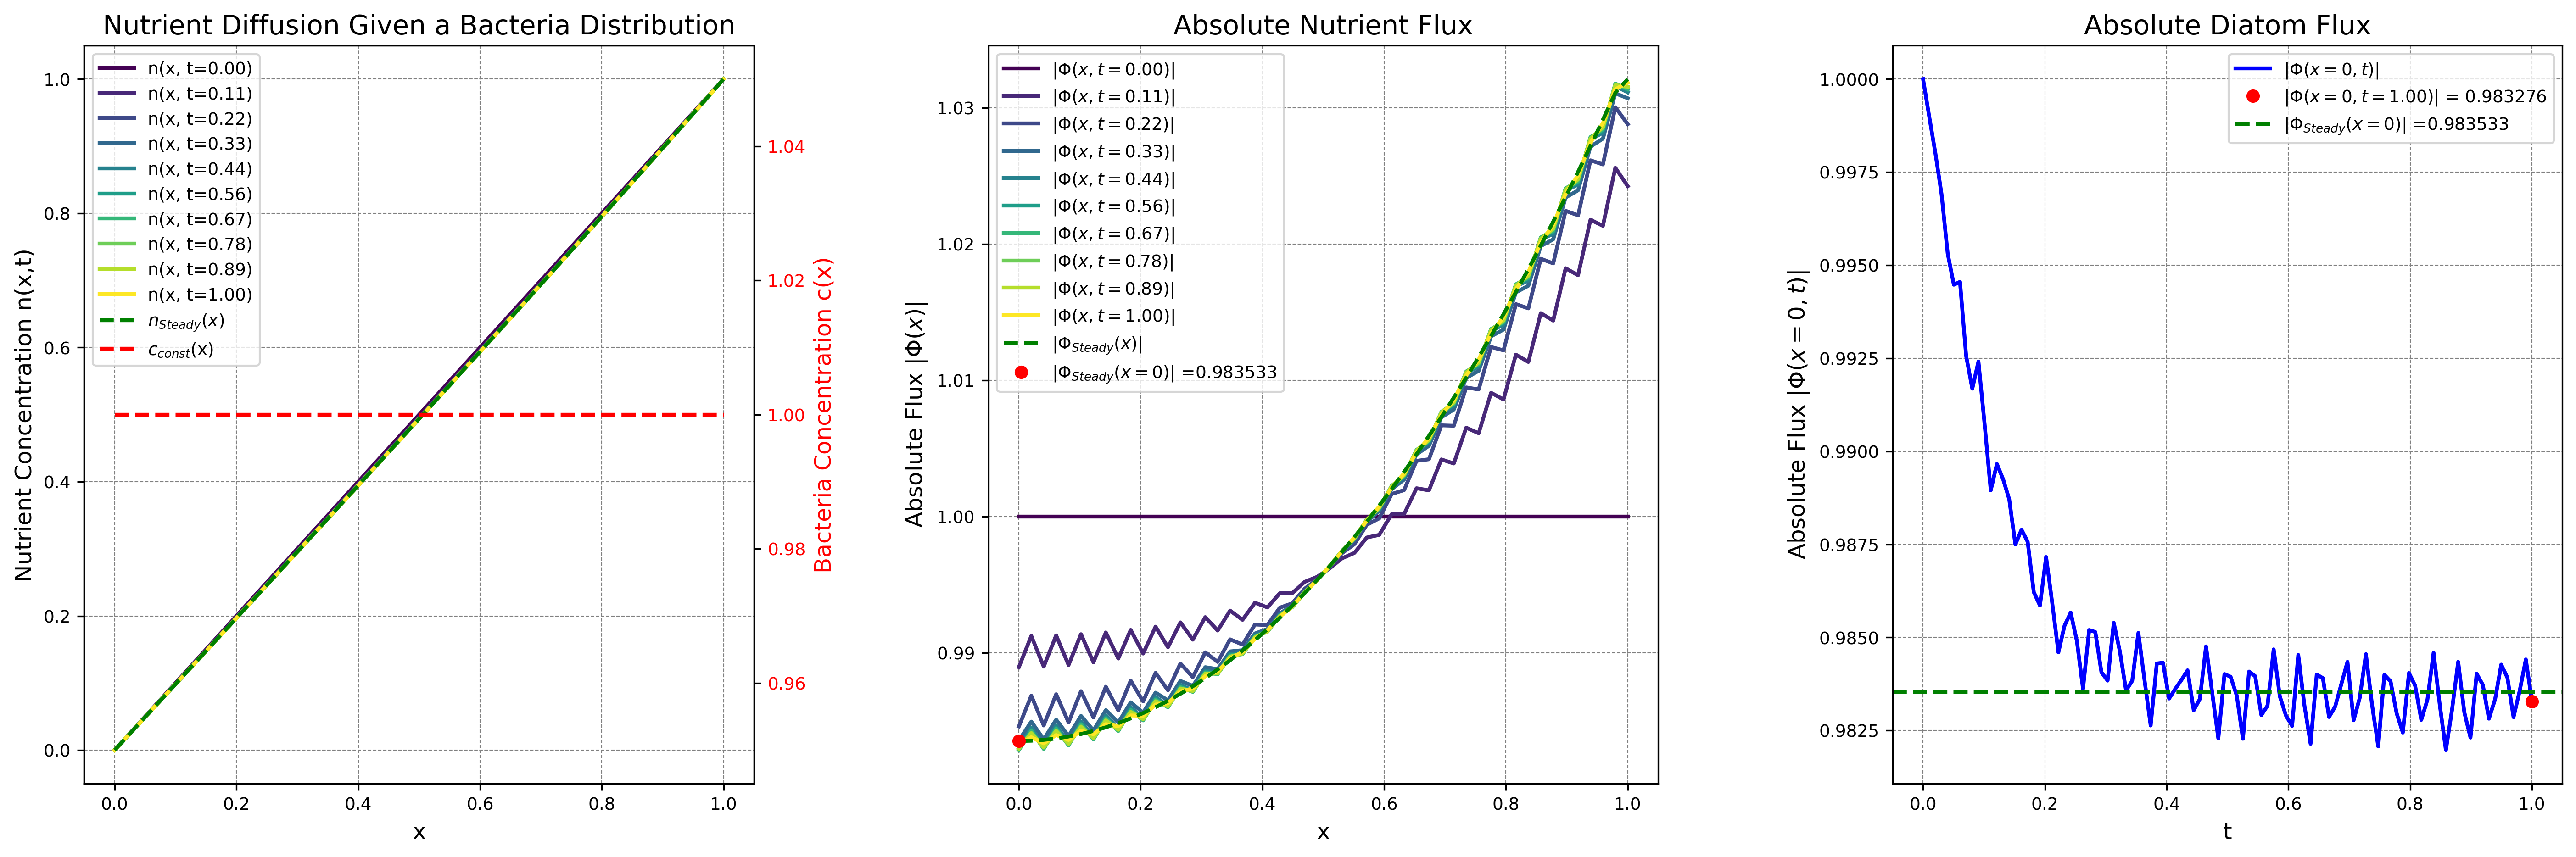
\includegraphics[width=0.8\textwidth]{Figures/Consump_Dom.png}
    \caption{Comparing Different Diffusion-Consumption Ratios.}
    \label{fig:Diff_Consump}
\end{figure}

\textbf{Diatom's FluxMaps, Generalising Results for Step \& Exponential Concentrations}

Concentration profile described by a midstep with varying starting positions ($x_0$) and lenghts ($l$), with the restriction $x_0 + l \leq L$.

\begin{equation}
    c_{\text{midstep}}(x; x_0,l) = 
    \begin{cases} 
    \frac{1}{l} & \text{if } x_0 \leq x \leq x_0 + l, \\
    0 & \text{otherwise}.
    \end{cases}
\end{equation}

\begin{figure}[H]
    \centering
    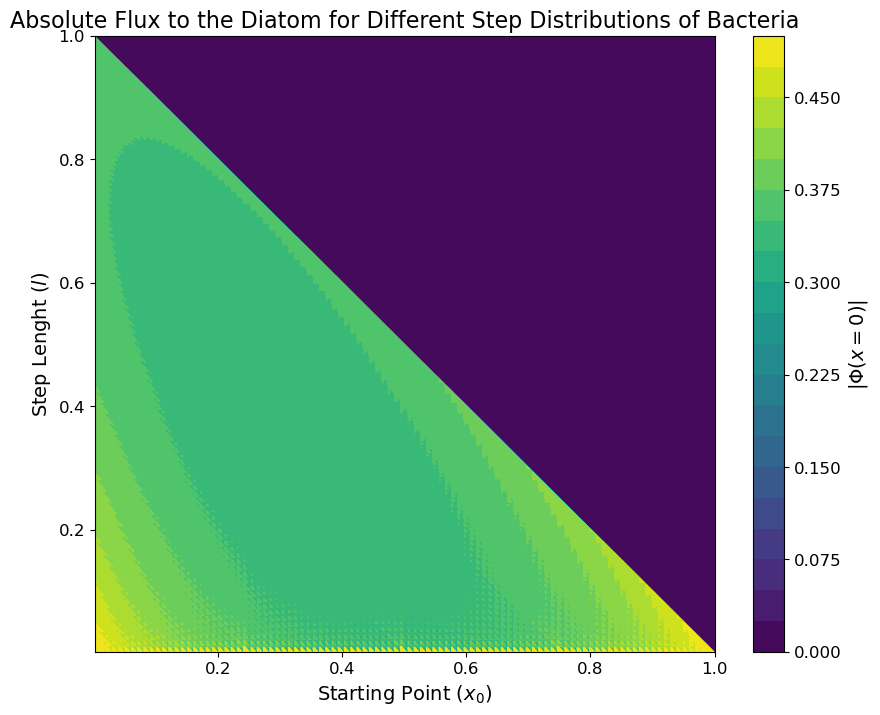
\includegraphics[width=0.6\textwidth]{Figures/FluxMap_midstep.png}
    \caption{Flux Map for Midstep Concentration Profile.}
    \label{fig:FluxMap_midstep}
\end{figure}

Concentration profile described by an exponential with varying slope.

\begin{equation}
    c_{\text{exp}}(x; \delta) =
    \frac{1}{\delta L}
    \frac{\mathrm{e}^{-\frac{x}{\delta L}}}{1 - \mathrm{e}^{-\frac{1}{\delta}}}
\end{equation}

\begin{figure}[H]
    \centering
    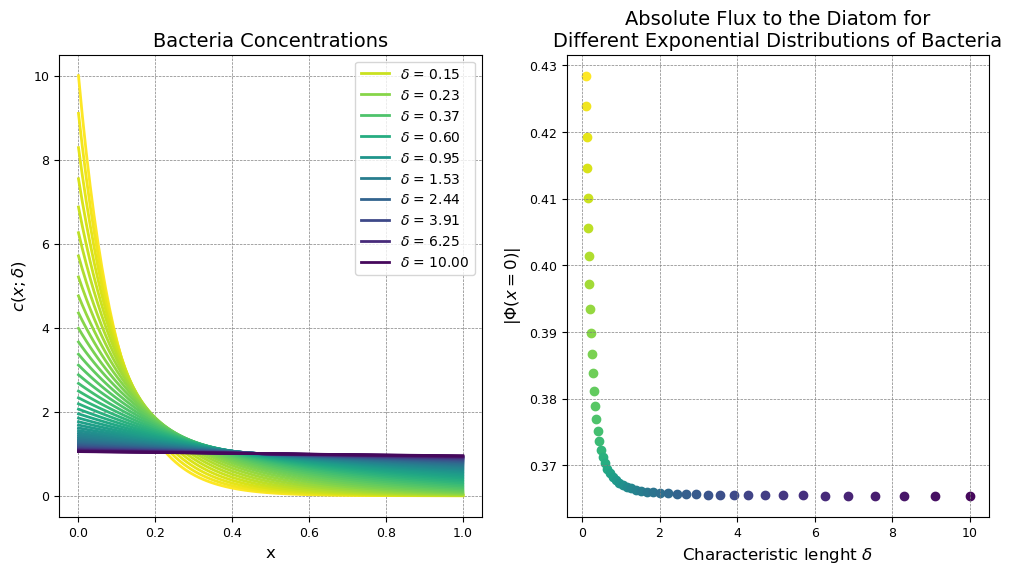
\includegraphics[width=0.6\textwidth]{Figures/FluxMap_exp.png}
    \caption{Flux Map for Exponential Concentration Profile.}
    \label{fig:FluxMap_exp}
\end{figure}

\subsubsection{Absorption of Brownian Particles}

\subsection{Tree-Dimensional Model}

\subsubsection{Numerical Solution}

\subsubsection{Analytical Solution}
    
    \section{Conclusion}
    \input{Sections/05.Conclusion.tex}

    \appendix
    \section{Coding Appendix}
    \subsection{Numerical Approach}

    
    \section{Mathematical Derivations}
    \input{Sections/B.Math.tex}
    
    % \printbibliography
\end{document}